\documentclass[11pt,a4paper]{article}
\usepackage[T1]{fontenc}
\usepackage[utf8]{inputenc}
\usepackage{lmodern}
\usepackage[margin=2.4cm]{geometry}
\usepackage{graphicx}
\usepackage{booktabs}
\usepackage{caption}
\usepackage{float}
\usepackage{enumitem}
\usepackage{parskip}
\usepackage[hidelinks]{hyperref}
\captionsetup{font=small, labelfont=bf}
\setlist{itemsep=2pt, topsep=4pt}
\graphicspath{{figures/}}

% ---- fill in before handing in ----
\newcommand{\teammembers}{Laurits Rossebø, Angelo Betza, Relja Savic}
\newcommand{\kagglenotebook}{\url{https://www.kaggle.com/code/lauritsrosseb/pokemon-battleprediction-final1}}
\newcommand{\githubrepo}{https://github.com/lauritsrossebo/fds-pokemon-battle-prediction}

\title{Predicting Pokémon Battle Outcomes from the First 30 Turns\\[4pt]
\large FDS Kaggle Challenge 2026, Sapienza University of Rome}
\author{\teammembers}
\date{November 2026}

\begin{document}
\maketitle
\vspace{-1.2em}
\begin{center}
\small Kaggle notebook: \kagglenotebook\\
Code: \url{\githubrepo}
\end{center}

\section{Introduction}

The task of the challenge is to predict whether Player~1 wins a Pokémon battle in the Generation~2
OverUsed format. For every battle we are given Player~1's full team of six, the lead Pokémon of
Player~2, and a turn-by-turn log of the first 30 turns: which Pokémon were active, their HP and
status, and the moves they used. The battles last between 30 and 80 turns, so in many of them more
than half of the game is still to be played when the log ends. There are 10,000 labelled training
battles and 5,000 test battles, the two classes are balanced, and the metric is accuracy.

Two things make the problem hard. First, we only see part of Player~2's team: a Pokémon appears in
the log only when it enters the field. Second, Gen~2 battles are slow and the lead changes often,
because of Leftovers, Rest and Spikes. The player who is ahead after 30 turns still loses a large
share of the battles.

Our final models are right in about 68--69\% of the battles. The three submissions we selected
scored between 0.6809 and 0.6820 on the private leaderboard (Table~\ref{tab:final}). This report
describes the stages we worked in, the features and models behind the three submissions, how we
validated them, and how the models behave when we look at more than their accuracy.

\begin{table}[H]
\centering\small
\begin{tabular}{@{}llccc@{}}
\toprule
\# & Model & 5-fold CV & Public & Private \\
\midrule
1 & LR + HGB blend on feature set B & 0.685 & 0.69333 & 0.68200 \\
2 & First version of the same blend & 0.689 & 0.69933 & 0.68114 \\
3 & Ensemble: LR + HGB on B, LightGBM + XGBoost on A & 0.688 & 0.69733 & 0.68085 \\
\bottomrule
\end{tabular}
\caption{The three final submissions. LR is logistic regression and HGB is scikit-learn's
HistGradientBoosting classifier.}
\label{tab:final}
\end{table}

\section{How we worked}

We did not follow one straight line. Team members worked on their own feature sets in parallel and
we combined the results in the last days. Looking back, the work had five stages.

\textbf{Stage 1: understanding the data and a baseline.} We started from the starter notebook, which
uses six average base stats of Player~1's team and Player~2's lead. With logistic regression this
gives 51.8\% in cross-validation, barely better than guessing. The team composition alone says
almost nothing about the winner, so the information had to come from the battle log. A first random
forest baseline reached 62.1\%.

\textbf{Stage 2: two feature sets.} Two feature sets were then developed independently. Feature
set~A describes the teams and the 30 turns with Gen~2 in mind (the 17 types, held items, special
attack and defence as separate stats). With a random forest it reached 66.8\%. Feature set~B was
built around one idea, replaying the log to reconstruct the state of every Pokémon at turn 30, and
reached 68.9\% with a blend of logistic regression and gradient boosting.

\textbf{Stage 3: combining the work.} We moved both feature sets into one Python package, replaced
the random forest on set~A by LightGBM and XGBoost, and tested two ways of combining the sets:
averaging models that are each trained on their own set, and training models on the union of all
524 columns.

\textbf{Stage 4: making the results reproducible.} When we regenerated the first blend on another
computer, about 3\% of the predictions changed although the code was the same. The cause was the
library versions (scikit-learn 1.7.2 against 1.9.1). We therefore recorded the library versions of every
submission, and the final notebook runs each submission with the versions it was made with. With
this, all three files are regenerated exactly.

\textbf{Stage 5: evaluation.} Finally we looked at the models beyond accuracy: ROC curves,
calibration, a learning curve, and how well cross-validation predicted the leaderboard
(Section~\ref{sec:evaluation}).

\section{Feature engineering}

Both feature sets use only the competition files. The table of species (base stats and types), the
species frequencies and the move vocabulary are built from the training file only.

\subsection{Feature set B: the state of the battle at turn 30 (233 features)}

The log shows only the two active Pokémon in each turn, but what happened to a Pokémon earlier
still counts after it is switched out. We therefore go through the 30 turns in order and keep the
last known HP and status of every Pokémon on both sides. Player~1's six Pokémon are known from the
start. Player~2's Pokémon are added when they first appear, and those that never appear are counted
as having full HP. From this replay we compute six groups of features:

\begin{itemize}
\item \textbf{State at turn 30:} fainted Pokémon, remaining team HP, Pokémon with low HP, status
counts, and the number of Pokémon that can still fight. Sleep caused by a Pokémon's own Rest is
counted separately from sleep caused by the opponent, since the first is a planned two-turn heal
and the second is a real disadvantage.
\item \textbf{Remaining strength:} the base stats of the Pokémon still alive, weighted by their HP.
\item \textbf{Momentum:} the difference in team HP at turns 10, 20 and 30, its mean, minimum and
maximum, and its slope over the 30 turns.
\item \textbf{How the battle went:} switches, turns without a move, damage dealt, stat boosts, the
use of moves that shape Gen~2 play (Spikes, Rapid Spin, Rest, Explosion, Curse and others), and the
power of the moves used, adjusted for STAB and for type effectiveness with the supplied type chart.
\item \textbf{Active Pokémon at turn 30:} HP, status, boosts, speed and type matchup of the two
Pokémon on the field.
\item \textbf{Team information:} base stats and types of Player~1's team and Player~2's lead, and
how common the species of each team are in the training data. A team of rarely used Pokémon may
indicate a less experienced player.
\end{itemize}

Most features exist for both players and as a difference (Player~1 minus Player~2), which the
linear model can use directly.

\subsection{Feature set A (291 features)}

Feature set A covers similar ground with a different implementation, and we kept both so that
models trained on each could be combined. It adds features that set~B does not have: counts of
sweepers and walls in each team, a team-against-team matchup based on STAB types, held items, the
HP healed during the 30 turns, the number of turns spent asleep, boosts per stat, the speed and
type matchups of the surviving Pokémon against the active opponent, and counts of the 60 most
common moves for each player.

\subsection{Feature selection}

We selected features by adding them in groups and keeping a group only if the cross-validated
accuracy improved. Table~\ref{tab:featexp} shows this for feature set~B. Indicator columns for the
species in each team, counts of every move and the remaining HP per species did not help, so they
were left out. All differences in the table are small compared with the variation between folds
(about 0.9 points), which told us early that the remaining errors were not a matter of a missing
feature group.

\begin{table}[H]
\centering\small
\begin{tabular}{@{}lccc@{}}
\toprule
Features & LR & HGB & Blend \\
\midrule
Battle state only (213) & 0.682 & 0.676 & 0.685 \\
+ team quality, Rest sleep against inflicted sleep & 0.683 & 0.678 & 0.684 \\
+ species indicators & 0.677 & 0.680 & 0.683 \\
+ counts of every move & 0.678 & 0.682 & 0.682 \\
+ remaining team strength (final set, 233) & 0.681 & 0.687 & 0.689 \\
+ remaining HP per species & 0.677 & 0.683 & 0.685 \\
\bottomrule
\end{tabular}
\caption{5-fold CV accuracy on feature set B when groups of features are added. Species indicators
and move counts were tested on top of the second row and then dropped; the last two rows build on
the second row.}
\label{tab:featexp}
\end{table}

\section{Models and submissions}

We used four models, all from classical machine learning:

\begin{itemize}
\item \textbf{Logistic regression} on standardised features with strong L2 regularisation
($C = 0.02$). Many features are correlated, for example HP totals and HP differences, and the
regularisation keeps the coefficients stable.
\item \textbf{HistGradientBoosting} (600 iterations, learning rate 0.03, 15 leaves, at least 50
samples per leaf, half of the features per split). Small trees and a low learning rate limit
overfitting on 10,000 battles.
\item \textbf{LightGBM} (800 trees, learning rate 0.02, 31 leaves, 30\% of the features per tree).
\item \textbf{XGBoost} (700 trees, learning rate 0.02, depth 4).
\end{itemize}

A blend is the plain average of the predicted probabilities, thresholded at 0.5. We used equal
weights: with differences this small, learned weights would mostly fit noise.

\textbf{Submission 2 (the first blend).} Logistic regression and HistGradientBoosting on feature
set~B. A linear model and a tree model make partly different errors: the blend scored 68.9\% in
cross-validation against 68.1\% and 68.7\% for its two members.

\textbf{Submission 1 (the blend, regenerated).} The same features and models, run again from the
shared package with newer library versions. It differs from submission~2 on 2.7\% of the test
battles and has a slightly better private score (0.68200 against 0.68114).

\textbf{Submission 3 (the merged ensemble).} The average of four models: logistic regression and
HistGradientBoosting on set~B, LightGBM and XGBoost on set~A. Each model keeps the feature set it
was tuned on. This was the best cross-validation score of the combined approaches (68.8\%).

Before these, we also submitted a random forest baseline, a random forest on feature set~A, and
LightGBM, XGBoost and logistic regression trained on the union of both feature sets. Their scores
are shown in Figure~\ref{fig:stages}.

\section{Validation}

All decisions were taken with stratified 5-fold cross-validation on the training set with fixed
seeds, repeated with a second seed for the final models. We kept the out-of-fold probabilities of
every model, so each training battle is predicted by a model that has not seen it, and a blend can
be scored on exactly the same folds as its members. The test set was only used to produce
predictions, and features and models were chosen on the cross-validation scores, not on the public
leaderboard.

The standard deviation of the accuracy between folds is 0.6 to 1.1 points. We used this as the
yardstick for every comparison: a change of less than about half a point was not treated as an
improvement.

\section{Evaluation}
\label{sec:evaluation}

The numbers and figures in this section are computed on the out-of-fold predictions for the
10,000 training battles. They are taken from the run of the Kaggle notebook.

\subsection{Metrics}

\begin{table}[H]
\centering\small
\begin{tabular}{@{}lccccc@{}}
\toprule
Model & Accuracy & ROC AUC & Log loss & Brier & F1 \\
\midrule
Starter baseline (6 features) & 0.5178 & 0.5195 & 0.6927 & 0.2498 & 0.5252 \\
Random forest (A) & 0.6706 & 0.7337 & 0.6042 & 0.2089 & 0.6735 \\
\midrule
Logistic regression (B) & 0.6813 & 0.7481 & 0.5918 & 0.2035 & 0.6847 \\
HistGradientBoosting (B) & 0.6876 & 0.7549 & 0.5839 & 0.2008 & 0.6903 \\
LightGBM (A) & 0.6812 & 0.7485 & 0.5916 & 0.2038 & 0.6830 \\
XGBoost (A) & 0.6806 & 0.7488 & 0.5892 & 0.2028 & 0.6846 \\
\midrule
Blend LR + HGB (submissions 1 and 2) & 0.6892 & 0.7581 & 0.5813 & 0.1994 & 0.6915 \\
Ensemble of the four models (submission 3) & 0.6883 & 0.7583 & 0.5808 & 0.1993 & 0.6912 \\
\bottomrule
\end{tabular}
\caption{Out-of-fold metrics (5-fold CV, seed 42), as computed in the Kaggle notebook. The letter
in brackets is the feature set. The CV scores in Table~\ref{tab:final} are the ones measured when
each submission was made, so they can differ from this table in the third decimal.}
\label{tab:metrics}
\end{table}

The single models are within 0.7 points of each other, whichever feature set they use, and the two
blends are a little better than every single model on all metrics (Table~\ref{tab:metrics}). The
gain from blending is small because the models largely agree: the correlation between the
predicted probabilities is about 0.90 for the two models on set~B, and about 0.92 between
HistGradientBoosting on set~B and LightGBM on set~A. The second feature set therefore adds little
that the first does not already contain. The
confusion matrix of the ensemble is balanced: 3,489 true and 1,606 false predictions of a
Player~1 win, 3,394 true and 1,511 false predictions of a loss. The model does not favour one
player.

\subsection{ROC curves and calibration}

\begin{figure}[H]
\centering
\begin{minipage}[t]{0.47\textwidth}\centering
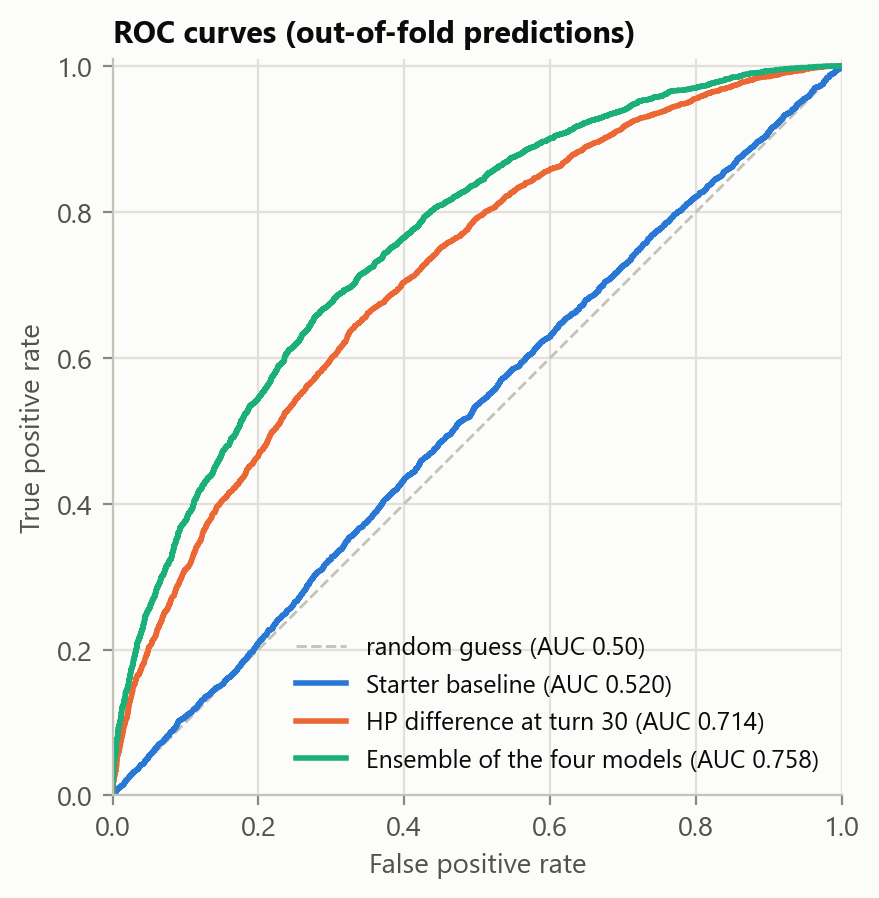
\includegraphics[width=\textwidth]{roc_curves.png}
\end{minipage}\hfill
\begin{minipage}[t]{0.51\textwidth}\centering
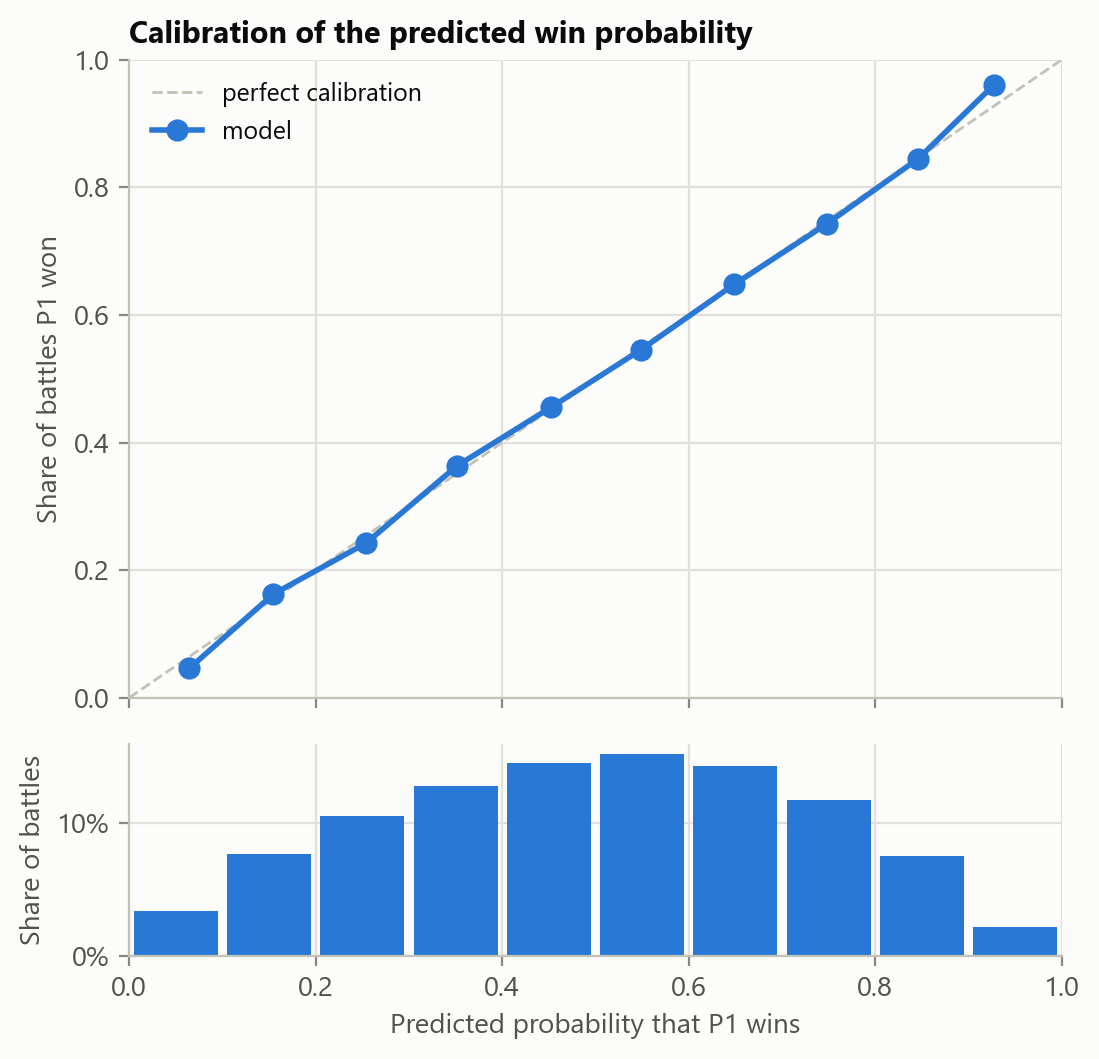
\includegraphics[width=\textwidth]{calibration.png}
\end{minipage}
\caption{Left: ROC curves of the starter baseline, of the HP difference at turn 30 used as a score,
and of the ensemble. Right: calibration of the ensemble. Each point is one tenth of the probability
range; the bars show how many battles fall in it.}
\label{fig:roc}
\end{figure}

Figure~\ref{fig:roc} (left) shows where the performance comes from. The starter baseline is almost
on the diagonal (AUC 0.52). A single number from the log, the difference in remaining team HP at
turn 30, already reaches an AUC of 0.71 and an accuracy of 63.1\%. All the other features and the
models together add about 4 points of AUC and almost 6 points of accuracy on top of it.

The predicted probabilities are well calibrated (Figure~\ref{fig:roc}, right): among the battles
where the ensemble gives Player~1 about 70\%, Player~1 won about 70\%. This matters for two
reasons. Averaging probabilities of different models is only sensible if they mean the same thing,
and a threshold of 0.5 is the right one for accuracy.

\subsection{Where the errors are}

\begin{figure}[H]
\centering
\begin{minipage}[t]{0.49\textwidth}\centering
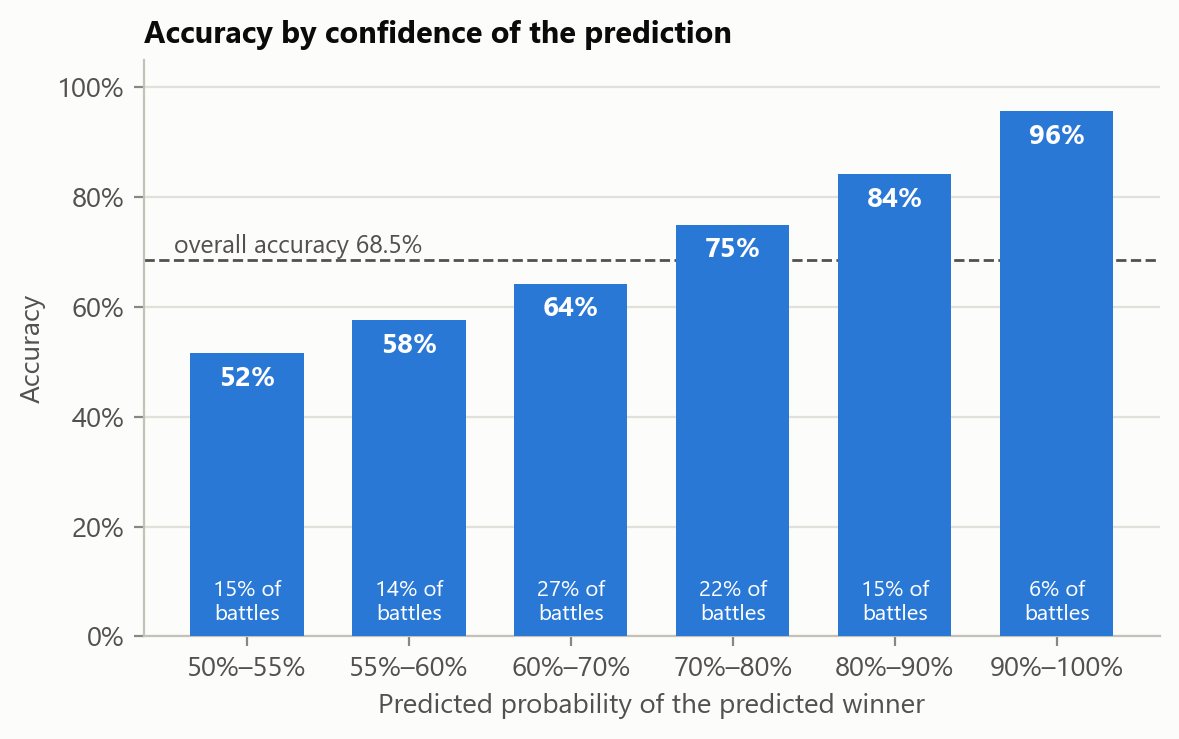
\includegraphics[width=\textwidth]{accuracy_by_confidence.png}
\end{minipage}\hfill
\begin{minipage}[t]{0.49\textwidth}\centering
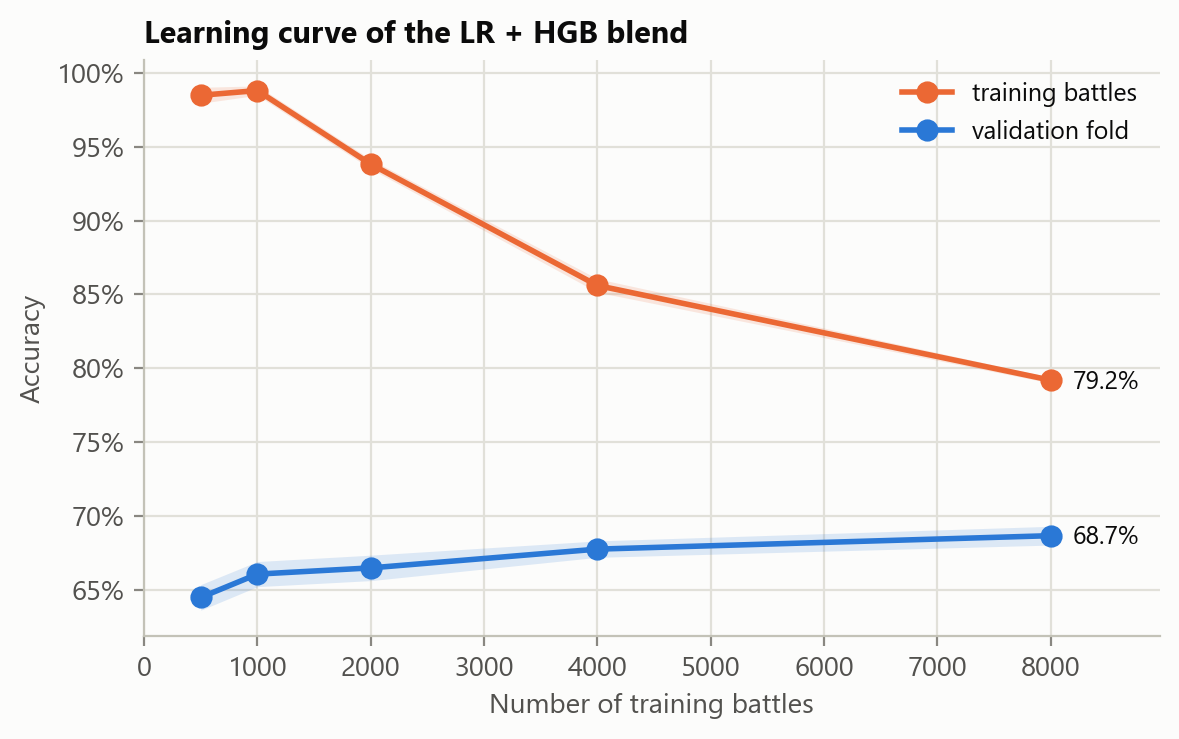
\includegraphics[width=\textwidth]{learning_curve.png}
\end{minipage}
\caption{Left: accuracy of the ensemble for battles grouped by the confidence of the prediction.
Right: learning curve of the LR + HGB blend (mean and standard deviation over five folds).}
\label{fig:conf}
\end{figure}

Because the model is calibrated, its confidence tells us which battles are hard
(Figure~\ref{fig:conf}, left). For the 21\% of battles where it is at least 80\% sure, it is
right in 85\% to 95\% of the cases. For the 30\% where it is below 60\%, it is right in only 53\%
to 58\%. These are battles that are still even after 30 turns, and their
result is decided in the turns we do not see. We think this, and not the choice of model, is what
limits the accuracy.

The learning curve (Figure~\ref{fig:conf}, right) supports this. The validation accuracy rises
from 64.8\% with 500 training battles to 68.9\% with 8,000, but the last doubling of the data adds
only about one point. The gap to the training accuracy (79.2\%) shows that the boosted trees still
overfit to some degree, even with small trees and regularisation. More battles would help a
little; a ten-point jump would need information that is not in the first 30 turns.

\subsection{What the linear model uses}

\begin{figure}[H]
\centering
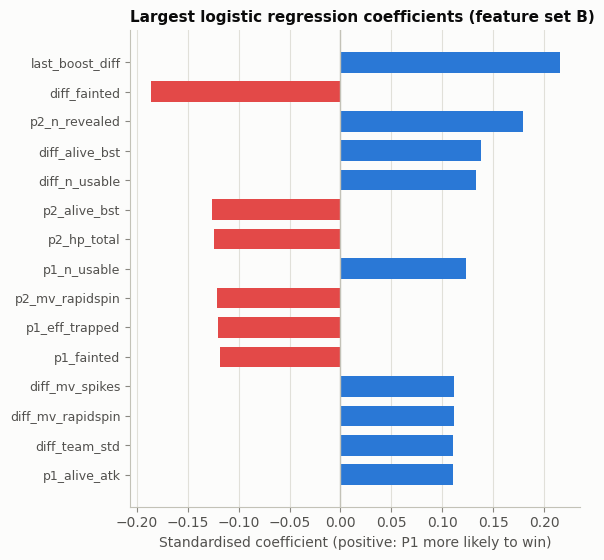
\includegraphics[width=0.62\textwidth]{top_coefficients.png}
\caption{The 15 largest standardised coefficients of the logistic regression on feature set B.}
\label{fig:coef}
\end{figure}

The largest coefficients (Figure~\ref{fig:coef}) are easy to interpret. Player~1 is more likely to
win when its active Pokémon has more stat boosts than the opponent's at turn 30, when it has lost
fewer Pokémon, and when its remaining team is stronger and has more Pokémon able to fight. Having
laid Spikes and having used Rapid Spin also count in a player's favour. One coefficient is less
obvious: the more of Player~2's team has been revealed, the better for Player~1, probably because
a player who is forced to switch a lot is under pressure.

\subsection{Cross-validation against the leaderboard}

\begin{figure}[H]
\centering
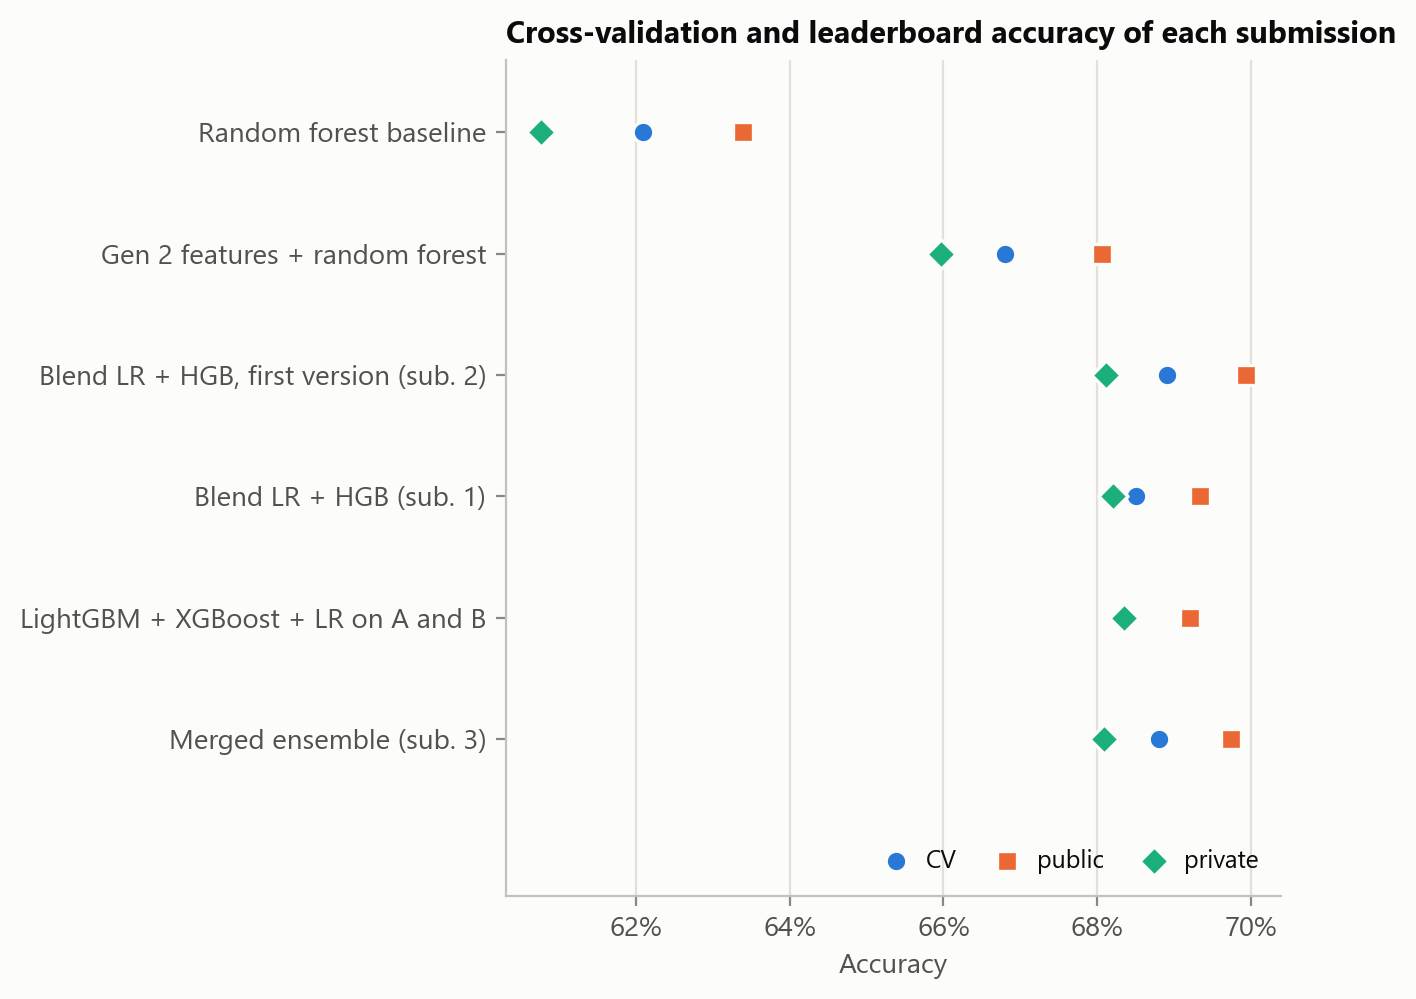
\includegraphics[width=0.78\textwidth]{scores_by_stage.png}
\caption{CV accuracy measured before submitting, and public and private leaderboard scores, for
all our submissions. We did not record a CV score for the model on the union of the feature sets.}
\label{fig:stages}
\end{figure}

Figure~\ref{fig:stages} compares the cross-validation estimate of every submission with its
leaderboard scores. Three things can be read from it.

\begin{itemize}
\item Cross-validation ranked the stages correctly: every large step in CV (from the random forest
baseline to feature set~A, and then to the blends) is also a large step on both leaderboards.
\item For the final models the CV estimate is 0.3 to 0.8 points above the private score, so it
was slightly optimistic but close. The public score is 0.9 to 2.6 points above the private score
for every submission, so the part of the test set behind the public leaderboard was simply a
little easier.
\item Among the last four models the differences are at most 0.4 points, on the private
leaderboard as well as in CV. That is below the variation between folds, so no validation scheme
could have ordered them reliably. The public leaderboard would have ordered them wrongly: our best
public score (submission~2) is not our best private score. The model on the union of the feature
sets, which is not one of our three final submissions, has the highest private score (0.68342),
0.14 points above submission~1.
\end{itemize}

\section{Conclusion}

Our best selected submission reaches 68.2\% on the private leaderboard with a blend of logistic
regression and gradient boosting on features that describe the state of both teams after 30 turns.

What worked:
\begin{itemize}
\item Replaying the log to keep the state of every Pokémon, instead of summarising only the active
ones. Features about remaining HP, fainted and usable Pokémon and the trend of the HP difference
carry most of the signal.
\item Blending a linear model with boosted trees. It gave a small but consistent gain, in
cross-validation and on every metric we looked at.
\item Using cross-validation and its fold-to-fold variation as the yardstick. It ranked our stages
correctly and showed that the differences among the final models were within noise.
\end{itemize}

What did not work: more columns. Species indicators, move counts, a second feature set and two more
boosting libraries all ended within a few tenths of a point of the first blend. Four different
models on two independently built feature sets reach the same accuracy, the models are well
calibrated, and their errors are concentrated in battles that are still even at turn 30. Our
conclusion is that the ceiling is set by the information in the first 30 turns more than by the
modelling.

If we continued, we would try to estimate Player~2's unseen Pokémon from the teams that usually
appear together in the training data, and separate chip damage (Spikes, poison, Leftovers) from
direct damage, since both would add information about the rest of the battle that the current
features do not have.

A practical lesson was reproducibility. The same code with other library versions changed
about 3\% of the predictions, which is more than the difference between our models. Recording
library versions from the first submission would have saved us work at the end.

\section*{Code and reproducibility}

The Kaggle notebook clones the repository linked on the first page and runs everything described
here: features, cross-validation, the evaluation figures and the three final submissions. Each
submission is generated in a separate process with the library versions it was originally made
with (\texttt{requirements/} in the repository), and the notebook compares the regenerated files
with the uploaded ones. In the run of the Kaggle notebook, all three regenerated files are
identical to the files we uploaded: 100\% of the 5,000 predictions are equal for each of them.

\end{document}
